\documentclass[18pt, twoside]{article}
\usepackage[utf8]{inputenc}
\usepackage{polski}
\usepackage{graphicx}
\graphicspath{ {./images/} }
\usepackage[margin=0.5in]{geometry}


\begin{document}
\begin{figure}[tp!]
	\center{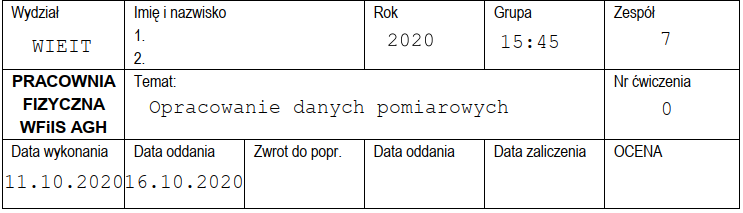
\includegraphics{F}}
\end{figure}

\begin{center}
	\section*{Opracowanie Danych Pomiarowych}
	\emph{Dzmitry Mikialevich}
\end{center}
\begin{center}
	\emph{Wojciech Sikora}
\end{center}
\tableofcontents
\newpage

\section{Wstęp}

    \subsection{Cel ćwiczenia}
    Zaznajomienie się z typowymi metodami opracowania danych pomiarowych
    przy wykorzystaniu wyników pomiarów dla wahadła prostego. 
    
    \subsection{Opis ćwiczenia}
    Zestawione wyniki opierają się na równaniu określającym zależność pomiędzy okresem drgań wahadła, oznaczonym jako \(T\), od długości wahadła \(l\) i przyśpieszenia ziemskiego \(g\).
    \[T = 2\pi \sqrt{\frac{l}{g}}\] \
    Powyższy wzór jest poprawny, gdy wychylenie środka ciężkości jest niewielkie.
    
\section{Układ Pomiarowy}
    \begin{enumerate}
    	\item Wachadło proste
    	\item Stoper
    	\item Linijka - (15cm:1mm)
    \end{enumerate}
\section{Przebiegi doświadczenia}
    Pomiar okresu drgań przy ustalonej długości wahadła:
    \begin{enumerate}
    	\item Mierzymy długość wahadła
    	\item Odchylenie wahadła na mały kąt i wprawienie go w ruch drgający
    	\item Pomiar czasu trwania k = 10 okresów
    	\item Wykonanie pomiaru N = 10 razy
    \end{enumerate}
    Pomiar okresu drgań przy zmiennej długości wahadła: 
    \begin{enumerate}
    	\item Mierzymy długość wahadła
    	\item Odchylenie wahadła na mały kąt i wprawienie go w ruch drgający
    	\item Pomiar czasu trwania k = 10 okresów
    	\item Wykonanie pomiaru N = 10 razy, zmieniając długość wahadła
    \end{enumerate}
\section{Wyniki Pomiarów}

    Długość wahadła: \[l= 45 cm = 450 mm \]\newline
    Niepewność pomiaru: \[ u(l) = 0,3cm = 3 mm \]
    {
    	\begin{table}[h]
    		\centering
    		\begin{tabular}{|l|l|l|l|}
    			\hline
    			
    			Lp. & Liczba okresów k & Czas t dla k okresów \([s]\) & okres \(T_i = t/k \)  \([s]\) \\ \hline
    			1   & 10                & 13,22                         & 1,322                         \\ \hline
    			2   & 10                & 13,62                         & 1,362                         \\ \hline
    			3   & 10                & 13,92                         & 1,392                         \\ \hline
    			4   & 10                & 13,37                         & 1,337                         \\ \hline
    			5   & 10                & 13,38                         & 1,338                         \\ \hline
    			6   & 10                & 13,28                         & 1,328                         \\ \hline
    			7   & 10                & 13,34                         & 1,334                         \\ \hline
    			8   & 10                & 13,35                         & 1,335                         \\ \hline
    			9   & 10                & 13,37                         & 1,337                         \\ \hline
    			10  & 10                & 13,45                         & 1,345                         \\ \hline
    		\end{tabular}
    		\textbf{\caption{Pomiar okresu drgań przy ustalonej długości wahadła  }
    		}
    	\end{table}}
    \newpage
    
    {
    	\begin{table}[h]
    		\centering
    		\begin{tabular}{|l|l|l|l|l|l|}
    			\hline
    			Lp. & l \([mm]\) & \(k\) & \(t[s]\) & \(T_i[s]\) & \(T_i^2[s^2]\) \\ \hline
    			1   & 280        & 10    & 10,23    & 1,023      & 1,047          \\ \hline
    			2   & 300        & 10    & 11,3     & 1,13       & 1,277          \\ \hline
    			3   & 310        & 10    & 11,72    & 1,172      & 1,374          \\ \hline
    			4   & 330        & 10    & 12,22    & 1,222      & 1,493          \\ \hline
    			5   & 340        & 10    & 12,35    & 1,235      & 1,525          \\ \hline
    			6   & 350        & 10    & 12,41    & 1,241      & 1,540          \\ \hline
    			7   & 360        & 10    & 12,52    & 1,252      & 1,568          \\ \hline
    			8   & 370        & 10    & 12,71    & 1,271      & 1,615          \\ \hline
    			9   & 400        & 10    & 12,96    & 1,296      & 1,680          \\ \hline
    			10  & 440        & 10    & 13,11    & 1,311      & 1,719          \\ \hline
    			11  & 450        & 10    & 13,31    & 1,331      & 1,772          \\ \hline
    			12  & 480        & 10    & 14,42    & 1,442      & 2,079          \\ \hline
    			13  & 500        & 10    & 14,43    & 1,443      & 2,082          \\ \hline
    			14  & 520        & 10    & 14,71    & 1,471      & 2,164          \\ \hline
    			15  & 550        & 10    & 15,7     & 1,57       & 2,465          \\ \hline
    		\end{tabular}
    		\textbf{\caption{Pomiar zależności okresu drgań od długości wahadła }
    		}
    	\end{table}}
 
\section{Opracowanie wyników Pomiarów}

    \subsection{Błędy grube}
    \textbf{Zadanie:} Oceń, czy wyniki pomiaru okresu nie zawierają błędów grubych. (Zwrócić uwagę na największą 
    i najmniejszą wartość \(T_i\) w uzyskanym zestawie danych):\newline
    Przy analizie wyników nie zauważyliśmy błędów grubych. Różnica między największą a najmniejszą wartością wynosi: \[\Delta t = t_{max} - t_{min} = 0,07s \]
    
    \subsection{Niepewność pomiaru okresu (typu A)}
    \textbf{Zadanie:} Oblicz niepewność pomiaru okresu (typu A): \newline
    \[u(T) =\sqrt{\frac{\sum{(T_i - \overline T)^2}}{n(n-1)}} = 0,0063s \approx 0,007s \] gdzie:  \(\overline T\) - średni okres, \(T_i\) - okres zmierzony za i-tym razem, \(n\) - liczba pomiarów
    
    \subsection{Niepewność pomiaru długości wahadła (typu B)}
    \textbf{Zadanie:} Oceń niepewność pomiaru długości wahadła (typu B):\newline 
    Podziałka linijki, za pomocą której było mierzone wahadło wynosi \(1mm\), jednak oszacowanie środka ciężkości stanowiło problem, w związku z trudnością wyznaczania środka masy, dlatego oszacowaliśmy niepewność typu B jako \(3mm\)
    
    \subsection{Przyspieszenie ziemskie  na podstawie uzyskanych wartości \(l\) i \(T\)}
    \textbf{Zadanie:} Na podstawie uzyskanych wartości l i T oblicz przyspieszenie ziemskie:\newline
    Korzystając ze wzoru na okres drgań wachadła matematycznego dla małych kątów odchylenia, mamy: \[T = 2\pi \sqrt{\frac{l}{g}} \Rightarrow g = \frac{4\pi^2}{T^2}l = \frac{4 \times 3,141^2}{(1,343s)^2} * 0,45m  \approx 9,846 m/s^2\]
    
    \subsection{Niepewność złożoną \(u_c(g)\) przy pomocy prawa przenoszenia niepewności}
    \textbf{Zadanie:} Oblicz niepewność złożoną \(u_c(g)\) przy pomocy prawa przenoszenia niepewności. \newline
    \[T = 2\pi \sqrt{\frac{l}{g}} \Rightarrow g = \frac{4\pi^2}{T^2}l  \Rightarrow \frac{\partial g}{\partial l} = \frac{4\pi^2}{T^2},\frac{\partial g}{\partial T} = -\frac{8\pi^2l}{T^3} \]
    \[u_c(g) = \sqrt{(\frac{\partial g}{\partial l} u(l))^2 + (\frac{\partial g}{\partial T} u(T))^2} = 
    	\sqrt{(21,87\times0,003)^2 + (14,65\times0,007)^2}
	 \approx 0,121 m/s^2\]
	Niepewność względna:
	\[\frac{u_c(g)}{g} * 100\% = 1,2\% \]
	Inny sposób wyliczenia, za pomocą współczynnika wrażliwości \(p_k\):
	\[\frac{u_c(g)}{g} = \sqrt{\sum_k ({p_k \frac{u(x_k)}{x_k})}^2}\]
	Gdzie: \[p_k = \frac{x_k}{y} \frac{\partial y}{\partial x_k} , p_l = 1 , p_T = -2\] 
	Czyli w końcu mamy:
	\[ \frac{u_c(g)}{g} = \sqrt{(1\times \frac{0,003}{0,45})^2 +(-2\times \frac{0,007}{1,343})^2 } \approx 1,2 \%\]
	\subsection{Niepewność rozszerzoną \(U(g)\)) przy pomocy prawa przenoszenia niepewności}
	\textbf{Zadanie:} Oblicz niepewność rozszerzoną U(g).\newline
	Niepewność rozszerzoną obliczamy za pomocą wzoru:
	\[U(g) = k \times u(g) = 0,242 m/s^2\]
	Gdzie:  \( k = 2\) - współczynnik rozszerzenia.
	Czyli mamy: \(g = 9,846 \pm  0,242 m/s^2\)
	
	\subsection{Porównanie uzyskanej wartości przyspieszenia ziemskiego z wartością tabelaryczną}
	\textbf{Zadanie:} Czy uzyskana wartość przyspieszenia ziemskiego jest zgodna, w granicach niepewności rozszerzonej, z wartością tabelaryczną? Dla Krakowa \(g = 9,811 m/s2\). \newline
	\[\Delta g = 9,846 m/s^2 - 9,8105 m/s^2 = 0,0355 m/s^2 < 0,242 m/s^2\] Czyli g mieści się w zakresie niepewności rozszerzonej:
	\[g_{otrz} \in (g-0,242m/s^2 , g+0,242m/s^2)\] Gdzie \(g=9,8105m/s^2\) - wartość przyspieszenia Ziemskiego w Krakowie.
	
	\subsection{Wykres zależności okresu od długości wahadła \(T(l)\)}
    %Tu TEKST
	\subsection{Wykres zlinearyzowany \(T^2\) w funkcji l}
	% Tu TEKST
	
	\subsection{Dopasowanie prostej typu \(y = ax\)}
	% Tu TEKST
	\subsection{Wartość przyspieszenia 
	ziemskiego z otrzymanej wartości współczynnika nachylenia}
	% Tu TEKST
	
	\subsection{Obliczanie niepewności u(g) z niepewności u(a) }
	% Tu TEKST
	\section{Wnioski}
	\begin{itemize}
	
    \item Biorąc pod uwagę, że przyjęliśmy dużą wartość błędu i brak dobrze skonfigurowanego wahadła, doświadczenie zostało wykonane poprawnie. To można podtwierdzić małą różnicą między wartością tabularną g a tą, którą otrzymaliśmy, która "mieści się" w niepewności rozszerzonej.
    \item Także eksperymentowow było podtwierdzone, że gdy maleje długość wahadła, również maleje okres T. 
    \item Liczyć niepewność względną jest wygodniej, korzystając z za pomocą współczynnika wrażliwości \(p_i\), co zmniejsza szansę na popełnienie błędów rachunkowych.
    \item Liczenie niepewności pozwala na oszacowanie rozrzutu wyników, co pomaga w dalniejszej analizie.
    \end{itemize}

\end{document}